\documentclass[letterpaper,12pt]{article}
\usepackage[margin=2cm]{geometry}

\usepackage{graphicx}
\usepackage[colorlinks=true]{hyperref}

\newcommand{\panhline}{\begin{center}\rule{\textwidth}{1pt}\end{center}}

\setlength{\parindent}{0em}

\title{\textbf{Safe Walk -- Gait Monitoring System\\\small (17S WSN Project)}}
\author{Emily Ruppel, Iljoo Baek, Mengwen He (Team 11)}

\begin{document}
\maketitle

\textbf{Introduction}\\
\href{../index.html}{Return}
\panhline
\section{Introduction}

\textbf{Difference in Gait}
\begin{figure}[!h]
	\centering
	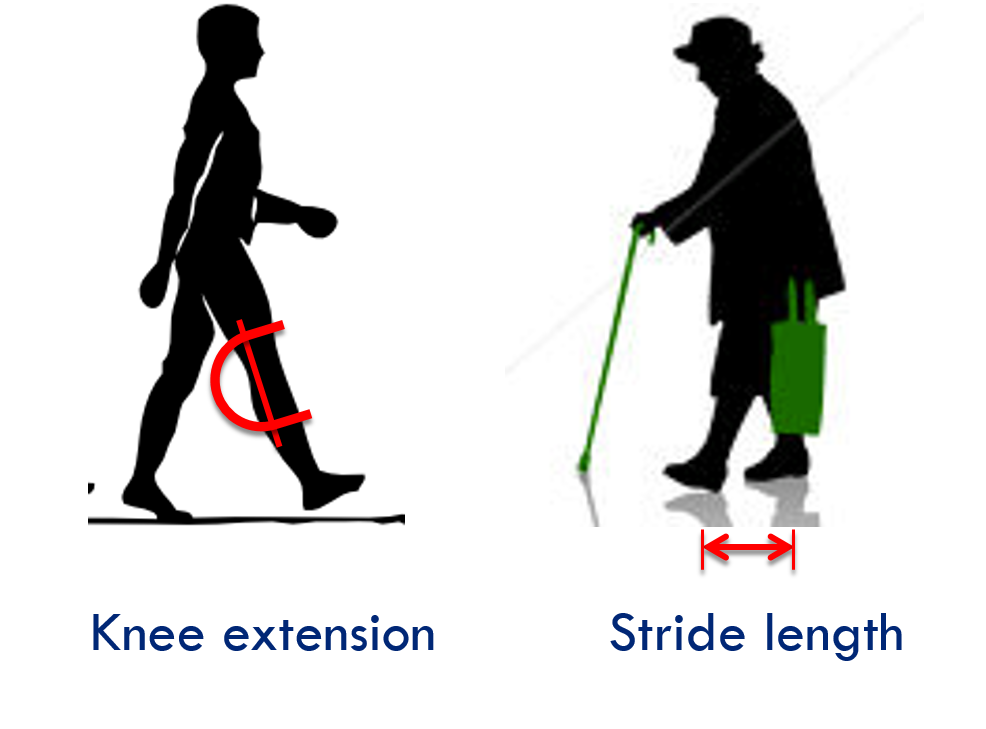
\includegraphics[width=15cm]{./imgs/gait.png}
\end{figure}

\textbf{Gait Data:}
\begin{itemize}
	\item Gait Speed
	\item Cadence
	\item Stride Length
	\item Double Stance Time
	\item Knee extension
	\item Swing Time
	\item Stride Length Variability
	\item Swing Time Variability 
	\item Cadence Variability	
\end{itemize}

\end{document}